\chapter{Vybrané zbernicové protokoly}
\label{kap:protokoly}

\section{Komunikácia s pamäťou AT93C66A}
Integrovaný obvod AT93C66A je jednoduchá pamäť typu EEPROM vyvinutá spoločnosťou Atmel. Veľkosť pamäte je 512 byte-ov, ktoré môžu byť organizované v 16-bitových slovách (words). Táto konfigurácia je nastaviteľná pomocou špeciálneho ORG pinu a je meniteľná za behu (atomicky vzhľadom na jednu inštrukciu) \cite{eepromDatasheet}.

\subsection{Inštrukčná sada}
AT93C66A je pamäť typu flash, preto rozlišuje dve rôzne operácie zápisu -- naprogramovanie (program) a zmazanie (erase). Naprogramovanie umožňuje nastavenie ktoréhokoľvek bitu vrámci adresovaného bloku (byte resp. slovo v závislosti od konfigurácie) na logickú hodnotu 0. Operácia zmazania umožňuje jednorázovo nastaviť celý adresovaný blok na logické hodnoty 1. 

Zápis do pamäte AT93C66A je preto možné realizovať pomocou dvoch inštrukcií. Inštrukcia ERASE umožňuje nastaviť všetky bity v jednom bloku pamäte (8 alebo 16 bitov v závislosti od konfigurácie pamäte) na logické hodnoty 1. Inštrukcia WRITE umožňuje zapísať do daného bloku ľubovoľnú hodnotu. V prípade, že pri zápise nie je potrebné vykonať zmenu bitu s hodnotou 0 na hodnotu 1, inštrukcia WRITE je interne realizovaná priamo operáciou naprogramovania. V opačnom prípade musí operácii naprogramovania predchádzať operácia zmazania, ktorú v tomto prípade pamäť implicitne vykoná, pred samotným zápisom (efektívne vykoná inštrukciu ERASE, pred samotnou inštrukciou WRITE). V tomto prípade možno očakávať, že operácia zápisu bude trvať dlhšie, podrobnosti však výrobca v technickom liste neuvádza. V obidvoch prípadoch výrobca garantuje, že inštrukcia WRITE trvá najviac 10\,ms \cite{eepromDatasheet}. Okrem spomenutých inštrukcií, obsahuje inštrukčná sada AT93C66A aj ďalšie inštrukcie, popísané v tabuľke \ref{tab:eepromIS}.

\begin{table}[!h]
    \caption[Inštrukčná sada pamäte AT93C66A]{Inštrukčná sada pamäte AT93C66A \cite{eepromDatasheet}. Veľkosť bloku závisí na konfigurácií organizácie -- 8/16 bitov.}
    \label{tab:eepromIS}
    \begin{center}
    \begin{tabular}{V{4}c|c|c|cV{4}}
        \hlineB{4}
        Inštrukcia & Kód & Operandy & Popis \\
        \hlineB{4}
        READ & 10 & adresa & Prečíta blok dát uložený na danej adrese. \\
        \hline
        WRITE & 01 & adresa a blok dát & Zapíše blok na danú adresu. \\
        \hline
        ERASE & 11 & adresa & Na danej adrese nastaví všetky bity na 1. \\
        \hline
        WRAL & 0001 & blok dát & Zapíše hodnotu bloku na každú adresu. \\
        \hline
        ERAL & 0010 & -- & Vymaže pamäť. (Nastaví všetky bity na 1). \\
        \hline
        EWEN & 0011 & -- & Povolí všetky zápisové operácie.\\
        \hline
        EWDS & 0000 & -- & Zakáže všetky zápisové operácie.\\
        \hline
        \hlineB{4}
    \end{tabular}
    \end{center}
\end{table}

\subsection{Zbernica a komunikačný protokol}
Rozhranie pre komunikáciu s pamäťou využíva SPI zbernicu, pričom vodiče sú v technickom liste (angl. datasheet) označené CS (Chip Select), DI (zodpovedá MOSI), DO (zodpovedá MISO) a SK (SCLK) \cite{eepromDatasheet}. V pasívnom stave je na linke CS logická 0, čo nie je v súlade s väčšinou implementácií SPI zbernice. (Pripomíname, že SPI zbernica je defakto štandard.) Frekvencia hodinového signálu na SK linke musí byť z rozsahu 0,25--2\,MHz \cite{eepromDatasheet}. Schéma vývodov (angl. pinout) je na obrázku \ref{obr:eepromPinout}.

\begin{figure}[h!]
    \centerline{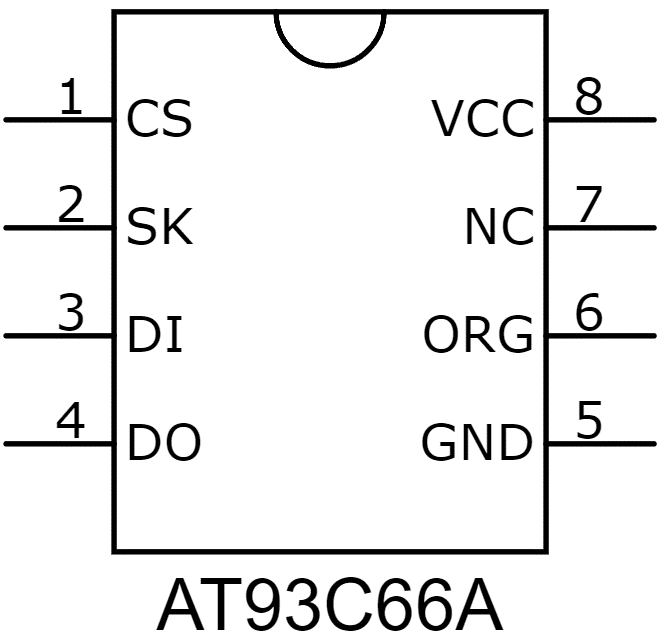
\includegraphics[width=0.25\textwidth]{images/at93c66aPinout.png}}
    \caption[Schéma vývodov pamäte AT93C66A]{Schéma vývodov pamäte AT93C66A. Pin NC (No Connect) je nevyužitý \cite{eepromDatasheet}.}
    \label{obr:eepromPinout}
\end{figure}

Komunikačný protokol pamäte je veľmi jednoduchý. Komunikácia je iniciovaná nábehovou hranou na CS vodiči a následným poslaním START bitu na DI. Na DI linke nasleduje kód inštrukcie a prípadné operandy (adresa a pri zápise aj obsah) \cite{eepromDatasheet}. V tabuľke \ref{tab:eepromIS} si možno všimnúť, že inštrukcie využívajú prefixový kód, čo umožňuje jednoznačne určiť inštrukciu a následne jej operandy, ktorých dĺžka už je jednoznačne určená z kontextu inštrukcie. Vstup (na DI linke) je vzorkovaný vždy s nábehovou hranou na SK linke s hodinovým signálom. Počas posielania inštrukcie musí byť na CS vodiči napätie na úrovni logickej 1.

Nasledujúca časť komunikácie závisí od zadanej inštrukcie. V prípade inštrukcie READ, začne pamäť posielať prečítané bity po DO linke hneď po zadaní inštrukcie (s nasledujúcou nábehovou hranou na SK linke). Výstup je synchronizovaný vždy s nábehovou hranou operácie čítania a predchádza mu jeden tzv. \uv{dummy} bit s hodnotou 0, ktorý sa na DO linke objaví súčasne s posledným bitom inštrukcie (v tomto prípade posledný bit zadanej adresy) na DI linke. Počas toho ako pamäť posiela výstup musí byť hodnota na CS vodiči rovná logickej 1. Po skončení operácie čítania musí napätie na CS vodiči klesnúť na úroveň logickej 0 a zotrvať minimálne po dobu 250\,ns, pred začatím ďalšej komunikácie. Komunikačný protokol v prípade inštrukcie READ je znázornený na obrázku \ref{obr:eepromREAD}. V prípade inštrukcie READ je možné ponechať napätie na CS linke na úrovni logickej 1 aj po prijatí posledného bitu prečítaných dát. V tom prípade s nasledujúcim taktom na SK linke začne pamäť automaticky posielať po DO linke obsah na nasledujúcej adrese. Takýmto spôsobom je možné sekvenčne prečítať pamäť až po poslednú adresu.

\begin{figure}
    \centerline{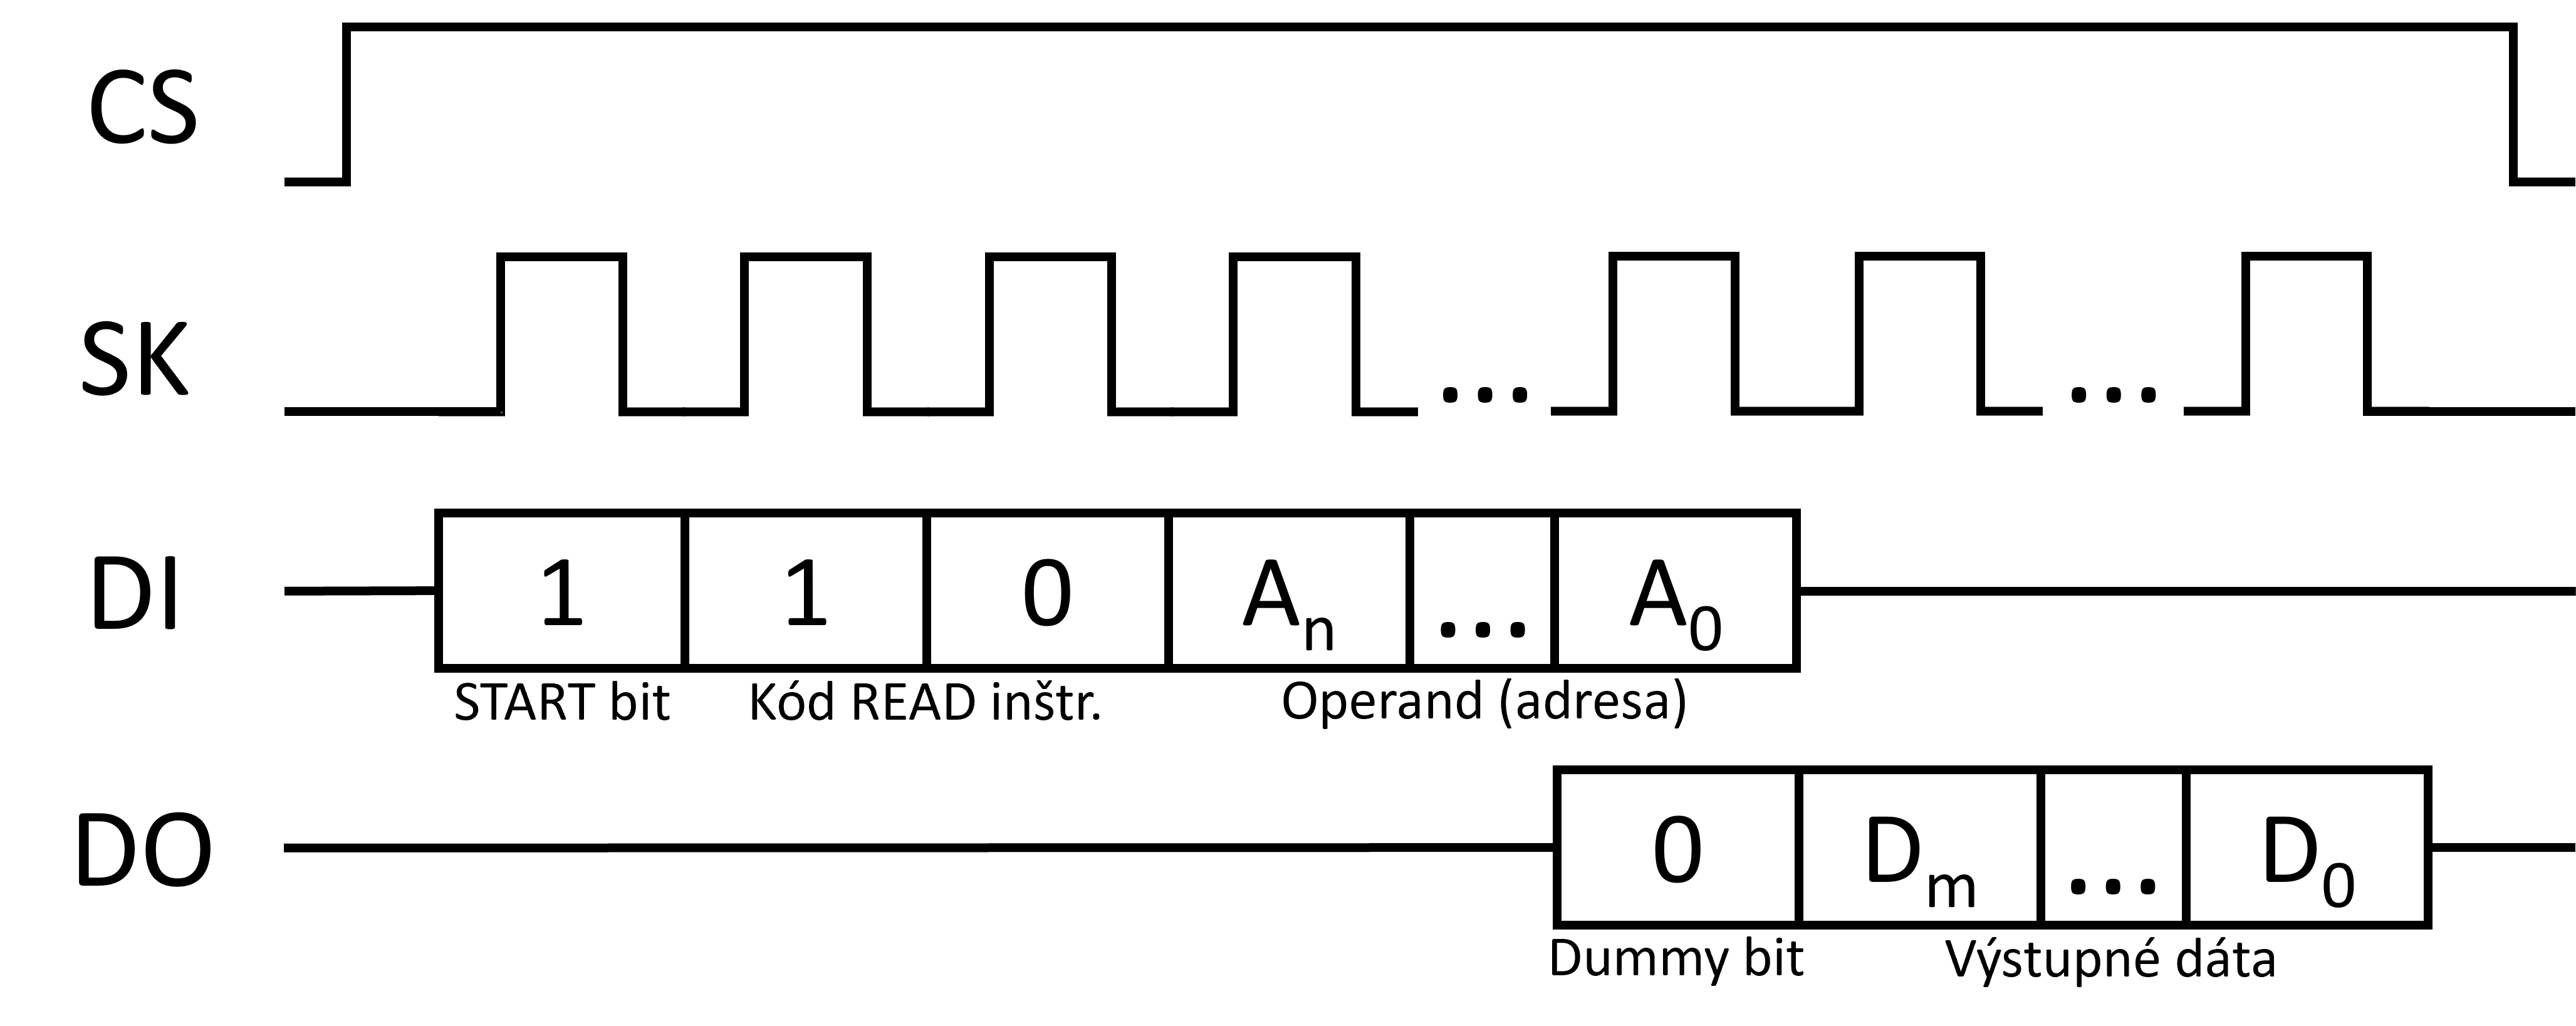
\includegraphics[width=1\textwidth]{images/eepromREAD.png}}
    \caption[Protokol pre čítanie pamäte AT93C66A]{Protokol pre čítanie pamäte AT93C66A. Na obrázku je znázornená komunikácia na jednotlivých linkách v čase. Adresa aj dáta sú posielané od najvyššieho bitu k najnižšiemu.}
    \label{obr:eepromREAD}
\end{figure}

V prípade inštrukcií zápisu WRITE, ERASE, WRAL a ERAL si pamäť vyhradzuje čas potrebný pre vykonanie inštrukcie (0,1 -- 10\,ms \cite{eepromDatasheet}). Tieto inštrukcie neprodukujú žiaden výstup, preto je komunikáciu možné ukončiť ihneď po zadaní inštrukcie nastavením logickej 0 na CS vodiči (minimálne po dobu 250\,ns ako v prípade READ inštrukcie). Pri nasledujúcej nábehovej hrane na CS vodiči (teda pokus o iniciovanie ďalšej komunikácie) začne pamäť na DO linke posielať tzv. READY/BUSY bit (synchronizovaný vždy na nábehovú hranu SK linky). Pokiaľ je pamäť pripravená na vykonanie ďalšej inštrukcie (READY), pošle bit s hodnotou 1, pokiaľ je zaneprázdnená (BUSY) vykonávaním predošlej inštrukcie, pošle bit s hodnotou 0. Takýmto spôsobom je možné opakovane testovať stav pamäte vždy s nábehovou hranou na SK linke. Počas tejto doby musí byť napätie na SC vodiči na úrovni logickej 1. Pokiaľ nábehová hrana na CS vodiči príde až po uplynutí vyhradeného času pre vykonanie inštrukcie, ktorý trvá minimálne 0,1\,ms, READY/BUSY komunikáciu už nie je možné iniciovať a pamäť očakáva ďalšiu inštrukciu. Opisaná komunikácia v prípade inštrukcií zápisu je znázornená na obrázku \ref{obr:eepromWRITE}.

\begin{figure}[h!]
    \centerline{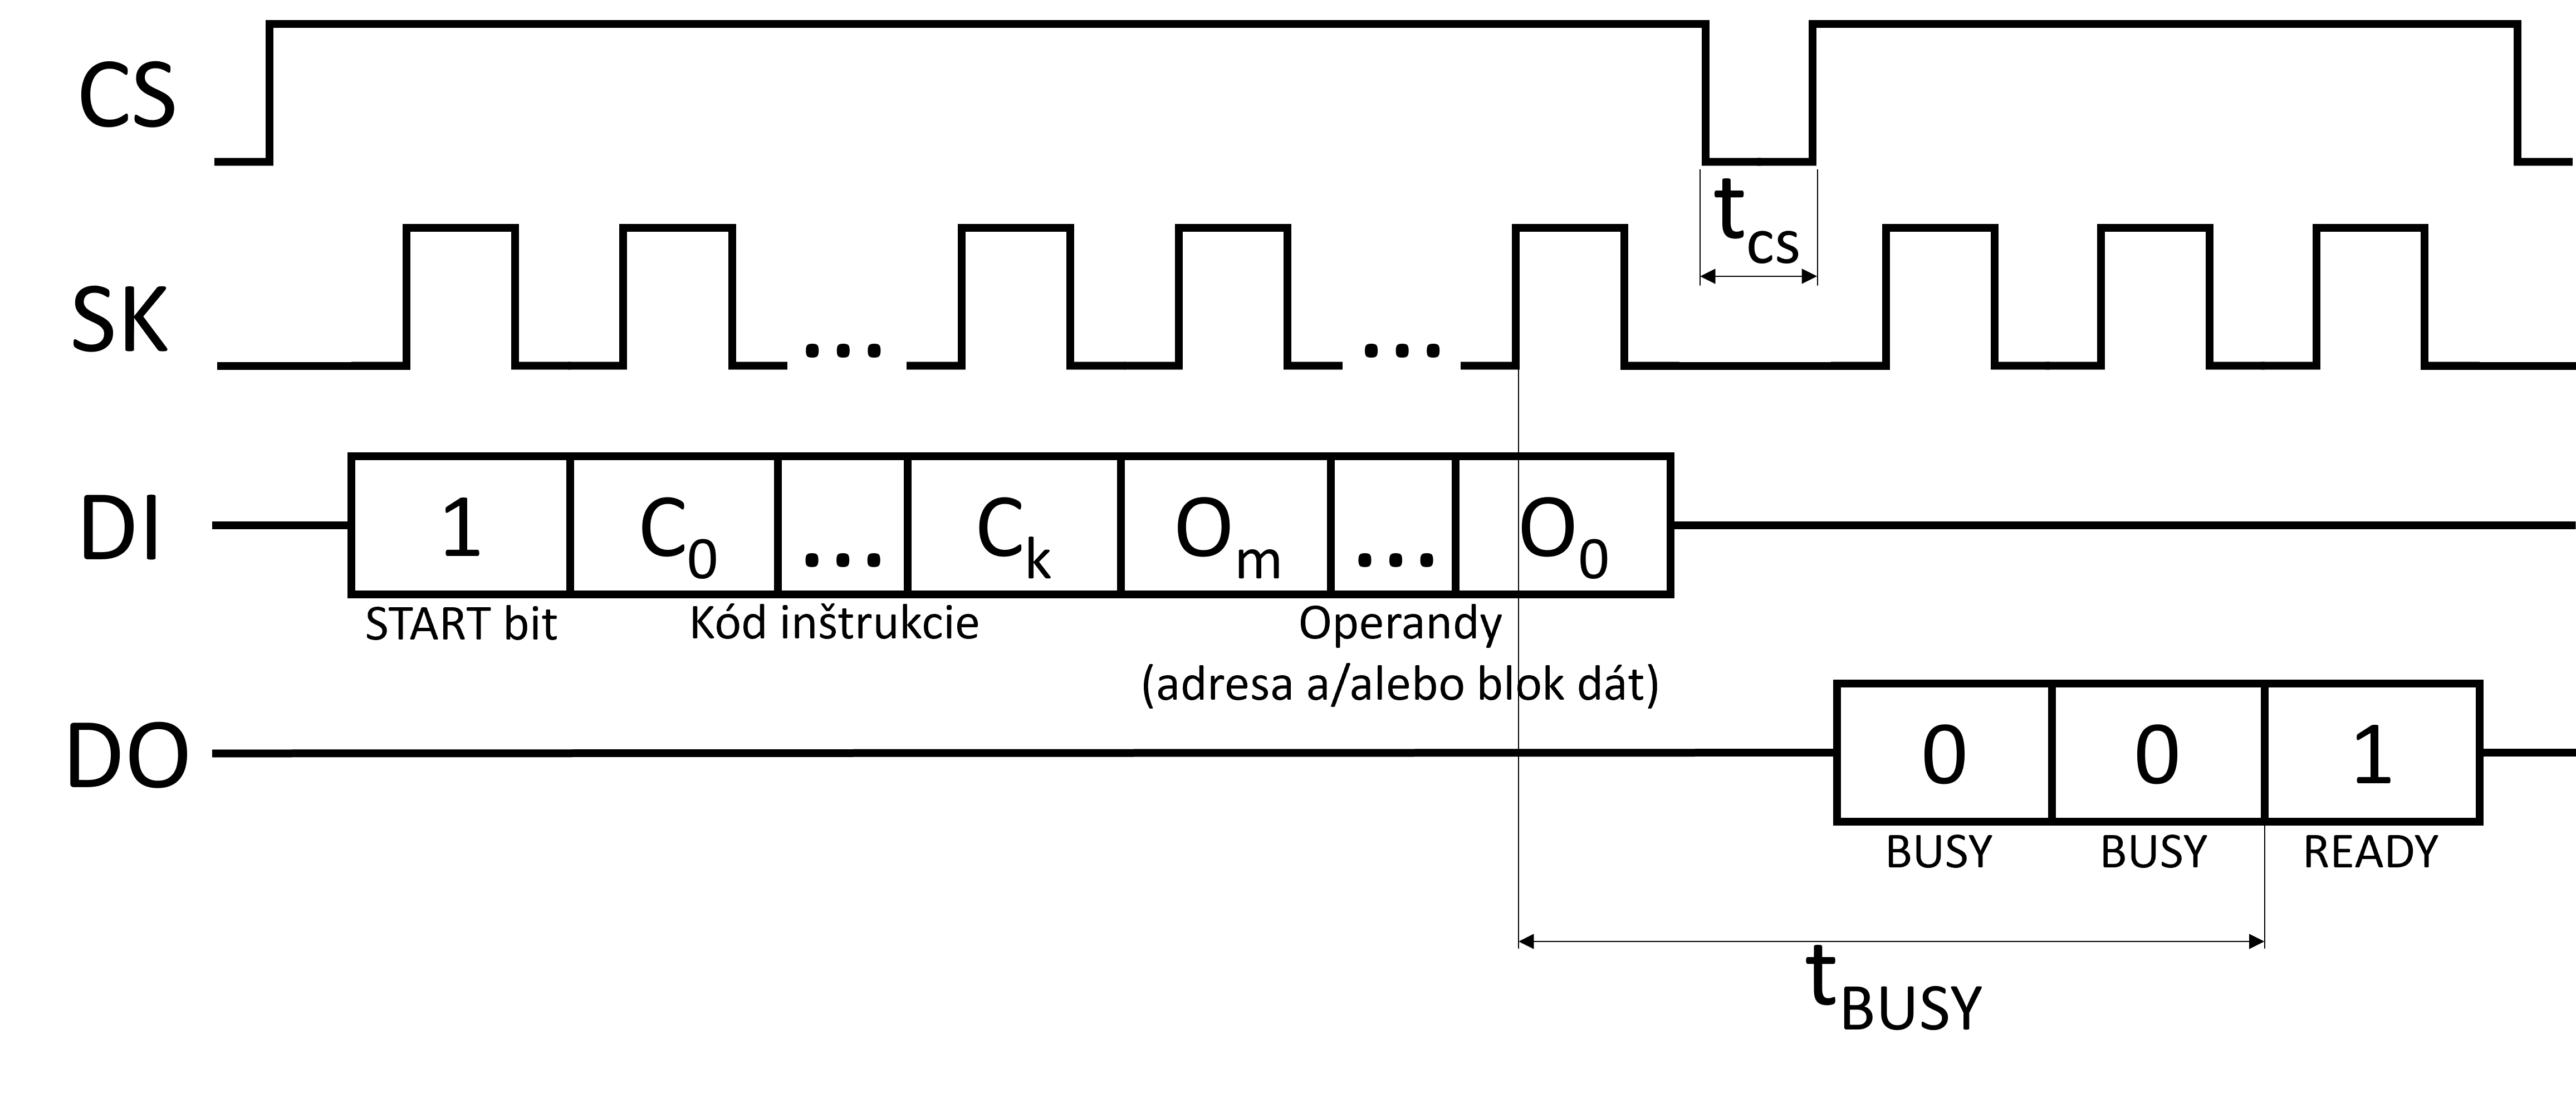
\includegraphics[width=1\textwidth]{images/eepromWRITE.png}}
    \caption[Protokol pre zápis do pamäte AT93C66A]{Protokol pre zápis do pamäte AT93C66A. Na obrázku je znázornená komunikácia na jednotlivých linkách v čase. Operandy sú posielané od najvyššieho bitu k najnižšiemu. Interval t\textsubscript{CS} je minimálne 250\,ns a t\textsubscript{BUSY} je z rozsahu 0,1 -- 10\,ms.}
    \label{obr:eepromWRITE}
\end{figure}

Inštrukcie EWEN a EWDS neprodukujú žiaden výstup a nevyhradzujú žiaden čas potrebný pre ich vykonanie. Po zadaní týchto inštrukcií preto možno komunikáciu ihneď ukončiť a následne iniciovať ďalšiu (opäť nastavením logickej 0 po dobu minimálne 250\,ns na CS vodiči). Z dôvodu zabezpečenia integrity dát sú po zapnutí napájania zakázané všetky inštrukcie zápisu (WRITE, ERASE, WRAL, ERAL). Inštrukcia EWEN musí byť preto vykonaná pred akoukoľvek inštrukciou zápisu. Po vykonaní inštrukcie EWEN sú inštrukcie zápisu povolené kým nebude vykonaná inštrukcia EWDS alebo do vypnutia napájania.